%%%%%%%%%%%%%%%%%%%%%%%%%%%%%%%%%%%%%%%%%%%%%%%%%%%%%%%%%%%%%%%%%
%  _____   ____  _____                                          %
% |_   _| /  __||  __ \    Institute of Computitional Physics   %
%   | |  |  /   | |__) |   Zuercher Hochschule Winterthur       %
%   | |  | (    |  ___/    (University of Applied Sciences)     %
%  _| |_ |  \__ | |        8401 Winterthur, Switzerland         %
% |_____| \____||_|                                             %
%%%%%%%%%%%%%%%%%%%%%%%%%%%%%%%%%%%%%%%%%%%%%%%%%%%%%%%%%%%%%%%%%
%
% Project     : LaTeX doc Vorlage für Windows ProTeXt mit TexMakerX
% Title       : 
% File        : header.tex Rev. 00
% Date        : 23.4.12
% Author      : Remo Ritzmann
% Feedback bitte an Email: remo.ritzmann@pfunzle.ch
%
%%%%%%%%%%%%%%%%%%%%%%%%%%%%%%%%%%%%%%%%%%%%%%%%%%%%%%%%%%%%%%%%%

\documentclass[ oneside,openright,titlepage,numbers=noenddot,headinclude,%1headlines,% letterpaper a4paper
                BCOR=5mm,paper=a4,fontsize=11pt,%11pt,a4paper,%
                ngerman,american,%
                ]{scrreprt}

%***********************************************************************
% include some libs
%***********************************************************************
\usepackage[utf8]{inputenc}
\usepackage{listings}
\usepackage{color}
\usepackage{fancyhdr}
\usepackage{rotating}
\usepackage{titlesec}
\usepackage{mathptmx}
% \usepackage{helvet}
\usepackage[scaled]{uarial}
\renewcommand*\familydefault{\sfdefault} %% Only if the base font of the document is to be sans serif
\usepackage[T1]{fontenc}
\usepackage{ngerman}
\usepackage{textgreek}
\usepackage{textcomp}
\usepackage[squaren]{SIunits}
\usepackage{graphicx}
\usepackage{url}
\usepackage{geometry}
\usepackage[absolute]{textpos}
\usepackage{makeidx}
\usepackage{colortbl}
\usepackage{pdflscape}
\usepackage{pdfpages}
\usepackage{tabularx}
\usepackage{lmodern}
\usepackage{longtable}
\usepackage{array}
\usepackage{float}
\usepackage{scrhack}
\usepackage[plainpages=false]{hyperref}
\usepackage{wallpaper} %\ThisTileWallPaper{}
%\usepackage[super,square]{natbib} für BibTeX Literaturverzeichnis
\usepackage{enumitem}
\usepackage{subfig}
\usepackage[export]{adjustbox}
\usepackage{setspace}
\usepackage{amsmath} 
\usepackage{fancyvrb}
\usepackage{graphicx}
\usepackage{booktabs}

% Bibliography
\usepackage[
backend=bibtex,
style=alphabetic-verb,
citestyle=alphabetic-verb
]{biblatex}
\bibliography{./Citer}

\usepackage{calc}



%***********************************************************************
% various styles
%***********************************************************************	

%create index
\makeindex

%define pagestyle
\pagestyle{fancy}

%use sans-serif font 
%\renewcommand{\familydefault}{\sfdefault}

%define page margin
\geometry{a4paper, top=30mm, left=30mm, right=30mm, bottom=30mm,headsep=10mm,footskip=10mm}

%textpos parameter
\setlength{\TPHorizModule}{30mm}
\setlength{\TPVertModule}{\TPHorizModule}
\textblockorigin{10mm}{10mm} % start everything near the top-left corner
\setlength{\parindent}{0pt}

%horizontal lines for titlepage 
\newcommand{\HRule}{\rule{\linewidth}{0.5mm}}

%reference to source items inlc source number
\newcommand{\srcref}[1]{\nameref{src:#1} \cite{#1}}

%header / footer 
\renewcommand{\headrulewidth}{0.3pt}
\renewcommand{\footrulewidth}{0.3pt}

\fancyhead[LO,RE]{} %clear headings for contents 

\fancyhead[RO,LE]{\nouppercase{\rightmark}} %right odd pages and left even pages
\fancyhead[LO,RE]{\MakeUppercase{\leftmark}} %left odd pages and right even pages
%\fancyhead[LO,RE]{\fontsize{9}{9}}
\fancyfoot[LE,RO]{\thepage} %page numbering
\fancyfoot[C]{} %clear centered page numbering 

%define some colors
\definecolor{gray}{rgb}{0.95,0.95,0.95}
\definecolor{darkgray}{rgb}{0.4,0.4,0.4}
%listing colors
\definecolor{lgray}{RGB}{250,250,250}
\definecolor{lgreen}{RGB}{63,127,95}
\definecolor{lred}{RGB}{127,0,85}
\definecolor{lblue}{RGB}{42,0,255}

%***********************************************************************
% listing
%***********************************************************************

\lstset{		
		basicstyle=\small\ttfamily,
		frame=single,
		numbers=left,	
		numberstyle=\tiny,
		%firstnumber=auto,
		numberblanklines=true,
		captionpos=b,
		extendedchars=true,
		float=ht,
		showtabs=false,
		tabsize=2,
		showspaces=false,
		showstringspaces=false,
		breaklines=true,
		%prebreak=\Righttorque,
		backgroundcolor=\color{lgray},
		keywordstyle=\color{lred}\bfseries, 
		commentstyle=\color{lgreen}\ttfamily,
%		morekeywords={printstr, printhexln},
		stringstyle=\color{lblue},
		xleftmargin=0.5cm,
		xrightmargin=0.5cm
}

\lstloadlanguages{R}

%\lstdefinelanguage{xc}{
%     keywords={printstr, printhexln, attributes, class, classend, do, empty, endif, endwhile, fail, function, functionend, if, implements, in, inherit, inout, not, of, operations, out, return, set, then, types, while, use},
%     keywordstyle=\color{lred}\bfseries,
%     ndkeywords={},
%     ndkeywordstyle=\color{yellow}\bfseries,
%     identifierstyle=\color{black},
%     sensitive=false,
%     comment=[l]{//},
%     commentstyle=\color{lgreen}\ttfamily,
%     string=[l]{"},
%     stringstyle=\color{lblue}\ttfamily
%  }




\begin{document}
%%%%%%%%%%%%%%%%%%%%%%%%%%%%%%%%%%%%%%%%%%%%%%%%%%%%%%%%%%%%%%%%%
%  _____   ____  _____                                          %
% |_   _| /  __||  __ \    Institute of Computitional Physics   %
%   | |  |  /   | |__) |   Zuercher Hochschule Winterthur       %
%   | |  | (    |  ___/    (University of Applied Sciences)     %
%  _| |_ |  \__ | |        8401 Winterthur, Switzerland         %
% |_____| \____||_|                                             %
%%%%%%%%%%%%%%%%%%%%%%%%%%%%%%%%%%%%%%%%%%%%%%%%%%%%%%%%%%%%%%%%%
%
% Project     : LaTeX doc Vorlage für Windows ProTeXt mit TexMakerX
% Title       : 
% File        : titlepage.tex Rev. 01
% Date        : 23.4.12
% Author      : Remo Ritzmann
% Feedback bitte an Email: remo.ritzmann@pfunzle.ch
%
%%%%%%%%%%%%%%%%%%%%%%%%%%%%%%%%%%%%%%%%%%%%%%%%%%%%%%%%%%%%%%%%%

\begin{titlepage}

% Logo
\ThisTileWallPaper{\paperwidth}{\paperheight}{images/logos/SoE.pdf} % {images/logos/*.pdf}
% Wählen Sie aus folenden pdf Files: ICP, IDP, IEFE, IMES, IMPE, IMS, INE, InES, InIT, KSR, SoE, ZAMP, ZAV, ZIL, ZPP, ZSN

\begin{minipage}[b]{0.117\textwidth}
\hskip 0.05cm
\end{minipage}
\begin{minipage}[b]{0.91\textwidth}
\begin{tiny}.\end{tiny}\vskip 2.8cm
	{\huge
	
	% Projekt Name
	\textbf{\underline{Bachelorarbeit (Informatikingenieurwesen)}}\\
	%\textbf{\underline{ }}
	
	% Projekt Titel
	Individuell Konfigurierbarer Authentifizierungsservice für Votings und Wettbewerbe
	\vskip 3.5cm}
	
	\begin{minipage}[b]{0.27\textwidth}
	\hrule\vskip 0.5cm
		\textbf{Autor}\\
		\\
	\end{minipage}
	\begin{minipage}[b]{0.03\textwidth}
	\hskip 0.5cm
	\end{minipage}
	\begin{minipage}[b]{0.7\textwidth}
	\hrule\vskip 0.5cm
	    Christian Bachmann\\
	    \\
	\end{minipage}
	
	\begin{minipage}[b]{0.27\textwidth}
	\hrule\vskip 0.5cm
		\textbf{Betreuung}\\
		\\
	\end{minipage}
	\begin{minipage}[b]{0.03\textwidth}
	\hskip 0.5cm
	\end{minipage}
	\begin{minipage}[b]{0.7\textwidth}
	\hrule\vskip 0.5cm
		Jaime Oberle\\
		 \\
	
	\end{minipage}
	
%	\begin{minipage}[b]{0.27\textwidth}
%	\hrule\vskip 0.5cm
%		\textbf{Nebenbetreuung}\\
%		\\
%	\end{minipage}
%	\begin{minipage}[b]{0.03\textwidth}
%	\hskip 0.5cm
%	\end{minipage}
%	\begin{minipage}[b]{0.7\textwidth}
%	\hrule\vskip 0.5cm
%		 keine\\
%		 \\
%	\end{minipage}
	
	\begin{minipage}[b]{0.27\textwidth}
	\hrule\vskip 0.5cm
		\textbf{Auftraggeber}\\
		\\
	\end{minipage}
	\begin{minipage}[b]{0.03\textwidth}
	\hskip 0.5cm
	\end{minipage}
	\begin{minipage}[b]{0.7\textwidth}
	\hrule\vskip 0.5cm
		inaffect AG\\
		\\
	\end{minipage}
	
%	\begin{minipage}[b]{0.27\textwidth}
%	\hrule\vskip 0.5cm
%		\textbf{Externe Betreuung}\\
%		\\
%	\end{minipage}
%	\begin{minipage}[b]{0.03\textwidth}
%	\hskip 0.5cm
%	\end{minipage}
%	\begin{minipage}[b]{0.7\textwidth}
%	\hrule\vskip 0.5cm
%		Elmer Melanie\\
%		Hürlimann Erich\\
%	\end{minipage}
	
	\begin{minipage}[b]{0.27\textwidth}
	\hrule\vskip 0.5cm
		\textbf{Datum}
	\end{minipage}
	\begin{minipage}[b]{0.03\textwidth}
	\hskip 0.5cm
	\end{minipage}
	\begin{minipage}[b]{0.7\textwidth}
	\hrule\vskip 0.5cm
		23.12.2015
	\end{minipage}
\end{minipage}
\vskip 0.5cm


%\textcolor{darkgray}{
%Bitte füllen Sie das Titelblatt aus und berücksichtigen Sie Folgendes:\\
% -> Bitte auf keinen Fall Schriftart und Schriftgrösse ändern. Text soll lediglich überschrieben werden!\\
% -> Bitte pro Tabellenzeile max. 4 Textzeilen!\\
%\\
%•	Vorlage: Haben Sie die richtige Vorlage gewählt? Logo Institut/Zentrum\\
%•	Titel: Fügen Sie Ihren Studiengang direkt nach dem Wort „Bachelorarbeit“ ein (max. 2 Zeilen).\\
%•	Titel der Arbeit: Überschreiben Sie den Lauftext mit dem Titel Ihrer Arbeit (max. 4 Zeilen).\\
%•	Autoren: Tragen Sie Ihre Vor- und Nachnamen ein (alphabetisch nach Name).\\
%•	Betreuer: Tragen Sie Ihren Betreuer / Ihre Betreuer ein (alphabetisch nach Name).\\
%•	Ohne Nebenbetreuung, Industriepartner oder externe Betreuung, ganze Tabellenzeile löschen.\\
%•	Datum: Aktuelles Datum eintragen.\\
%•	Am Schluss löschen Sie den ganzen Beschrieb (grau) und speichern das Dokument als pdf. ab.
%}


\end{titlepage}



% We will generate all images so they have a width \maxwidth. This means
% that they will get their normal width if they fit onto the page, but
% are scaled down if they would overflow the margins.
\makeatletter
\def\maxwidth{\ifdim\Gin@nat@width>\linewidth\linewidth
\else\Gin@nat@width\fi}
\makeatother
\let\Oldincludegraphics\includegraphics
\renewcommand{\includegraphics}[1]{\Oldincludegraphics[width=\maxwidth]{#1}}

\VerbatimFootnotes

\setlength{\parindent}{0pt}
\setlength{\parskip}{6pt plus 2pt minus 1pt}
\setlength{\emergencystretch}{3em}  % prevent overfull lines
\providecommand{\tightlist}{%
  \setlength{\itemsep}{0pt}\setlength{\parskip}{0pt}}
\VerbatimFootnotes % allows verbatim text in footnotes

\title{Projektarbeit: Projektkennzahlen}
\author{Reto Spaltenstein, Christian Wyder}



\setcounter{page}{1}


%Inhaltsverzeichnis
\tableofcontents
\newpage

\part[Präambel]{Einleitung und Abgrenzung}

\chapter{Einführung}\label{einfuxfchrung}

\section{Motivation und
Fragestellung}\label{motivation-und-fragestellung}

Der Zugriff auf Services und Medien mittels mobiler Geräte steigt
beständig an. So ist im Mai 2014, 60\% der Zeit, die online verbracht
wird, über Handy und Tablet zugegriffen worden - davon 51\% mittels
mobiler Applikationen. (Lipsman 2014)

\newpage

\chapter{Recherche}\label{recherche}

\section{Fachbegriffe}\label{fachbegriffe}

Eine ausführliche Erklärung der Fachbegriffe befindet sich im Anhang
unter dem Kapitel ``\protect\hyperlink{glossar}{Glossar}''.

\section{Erläuterung der
Grundlagen}\label{erluxe4uterung-der-grundlagen}

In diesem Kapitel werden Funktionsweisen und Grundlage ausgeführt, die
als für die Bearbeitung dieser Bachelorthesis herangezogen wurden.

\subsection{Authentifizierung}\label{authentifizierung}

Authentifizierung - beglaubigen, die Echtheit von etwas bezeugen
verfolgt das Ziel (\emph{Duden} 2014)

Eine Person oder Objekt eindeutig zu \textbf{authentifizieren} bedeute
zu ermitteln ob die oder derjenige auch der ist als welcher er sich
ausgibt. (Rouse 2015) Dies unterstreicht auch die Ableitung des Wortes
vom Englischen Verb \emph{authenicate}, was auf Deutsch sich als
\emph{echt erweisen, sich verbürgen, glaubwürdig sein} bedeutet. Das
bekannteste Verfahren der Authenfizierung ist die Eingabe von
Benutzernamen und Passwort. Weiter ist die PIN-Eingabe bei Bankautomaten
oder Mobiletelefon häufig verbreitet. Die Möglichkeiten der
Authentifizierung nahe zu grenzenlos. (``Http://authentifizierung.org''
2015)

\subsection{Autorisierung}\label{autorisierung}

Autorisierung - Befugnis, Berechtigung, Erlaubnis, Genehmigung
(\emph{Duden} 2014)

Wenn die
Authenfizierung\protect\hyperlink{authentifizierung-1}{Authentifizierung}
erfolgreich war erteilt das System die Autorisierung. Dabei wird der
Person oder Objekt erlaubt bestimmte Aktionen/Zugriffe durchzuführen.
Meist verfügen unterschiedliche Benutzer eines Systems über verschiedene
Zugriffsrechte. Die korrekte Zuweisung der individuellen Rechte ist
ebenfalls Bestandteil der Autorisierung.

Der Begriff Authentifizierung wird vielfach mit dem Begriff
Autorisierung verwechselt. Die Authentifizierung wird vom Benutzer
initiiert. Sie dient dem Nachweis, zur Ausübung bestimmter Rechte befugt
zu sein. Die anschließende Autorisierung erfolgt automatisch durch das
System selbst. Im Zuge der Autorisierung werden dem Benutzer seine
Zugriffsrechte zugewiesen. (``Http://authentifizierung.org'' 2015)

\subsection{Captcha}\label{captcha}

Captcha - Test, mit dem festgestellt werden kann, ob sich ein Mensch
oder ein Computer eines Programms bedient (\emph{Duden} 2014)

Im Jahre 2000 wurde das Captcha an der Carnegie Mellon University
erfunden. Captcha steht für \textbf{C}ompletely \textbf{A}utomated
\textbf{P}ublic \textbf{T}uring test to tell \textbf{C}omputers and
\textbf{H}umans \textbf{A}part. Luis von Ahn, Professor der
Entwickler-Gruppe, erklärte die Dringlichkeit von Captcha damals so:
``Anybody can write a program to sign up for millions of accounts, and
the idea was to prevent that''. (Burling 2012)

\subsubsection{Captcha Zahlen}\label{captcha-zahlen}

In 2014 wurden 200 Million Captchas pro Tag eingegeben. Dabei braucht
ein User durchschnittlich 10 Sekunden das entspricht 500'000
Stunden.\footnote{Die statistischen Daten wurden von Google 2014 in
  ihrem Blog publiziert (``ReCAPTCHA Digitization Accuracy'' 2014)}

\begin{figure}[htbp]
\centering

\includegraphics{images/captcha.png}
\caption{Beispiele von Captchas \emph{Quelle:drupal.org}}
\end{figure}

\newpage

\hypertarget{oauth}{\subsection{OAuth}\label{oauth}}

OAuth ist ein Protokoll. Es erlaubt sichere API-Autorisierungen.

\subsubsection{Das Bedürfnis nach
OAuth}\label{das-beduxfcrfnis-nach-oauth}

2006 implementiere Blaine Cook OpenID für Twitter und Ma.gnolia erhielt
ein Dashboard welches sich durch OpenID autorisieren lies. Deshalb sich
die Entwickler von Ma.gnolia und Blaine Cook um eine Möglichkeit zu
finden OpenID auch für die Verwendung von APIs zu gebrauchen. Sie
diskutierten ihre Implementierungen und stellten fest das es keinen
offenen Standart für API-Access Delegation gab. So fingen sie an den
Standart zu entwickeln. 2007 entstand daraus eine Google Group. Am 3.
October 2007 war dann der OAuth Core 1.0 bereits released worden.

\subsubsection{Funktionalität von
OAuth}\label{funktionalituxe4t-von-oauth}

Ein Programm/API (Consumer) stellt über das OAuth-Protokoll einem
Endbenutzer(User) Zugriff (Autorisierung) auf seine
Daten/Funktionalitäten zur Verfügung. Dieser Zugriff wird von einem
anderen Programm (Service) gemanagt. Das Konzept ist nicht generell neu.
OAuth ist ähnlich zu Google AuthSub, aol OpenAuth, Yahoo BBAuth,
Upcoming api, Flickr api, Amazon Web Services api. OAuth studierte die
existierenden Protokolle und standardisiert und kombinierte die
existierende industriellen Protokolle. Der wichtigste Unterschied zu den
existierenden Protokollen ist, das OAuth sowohl offen ist und anderseits
zu einem Standard geworden ist. Jeden Tag entstehen neue Webseite welche
neue Funktionalitäten und Services offeriert und dabei Funktionalitäten
von anderen Webseiten braucht. OAuth stellt dem Programmierer einerseits
eine standartisierte Implementierung zur Verfügung. Der Endbenutzer
erhält dank dieses Protokoll die Möglichkeit teile seiner
Funktionalität/Daten bei einem anderen Anbieter zur Verfügung zu
stellen. So kann der Endbenutzer bei der Facebook OAuth z.b. seine Posts
zur Verfügung stellen nicht aber seine Freunde bekannt geben.

Dank der weiten Verbreitung gibt es nun in allen bekannten
Programmiersprachen eine Implementierung sowohl von Client wie auch vom
Server. Weitere Infos dazu unter oauth.net\href{http://oauth.net/2/}{1}

\newpage

\section{Ähnliche Produkte auf dem
Markt}\label{uxe4hnliche-produkte-auf-dem-markt}

Dieses Unterkapitel erläutert existierenden Produkte auf dem Markt.

\subsection{OAuth-Provider}\label{oauth-provider}

Die grössten \protect\hyperlink{oauth}{OAuth}-Provider wie Google,
Facebook und Twitter erziehlen eine weiter Verbreitung weltweit:

\begin{figure}[htbp]
\centering
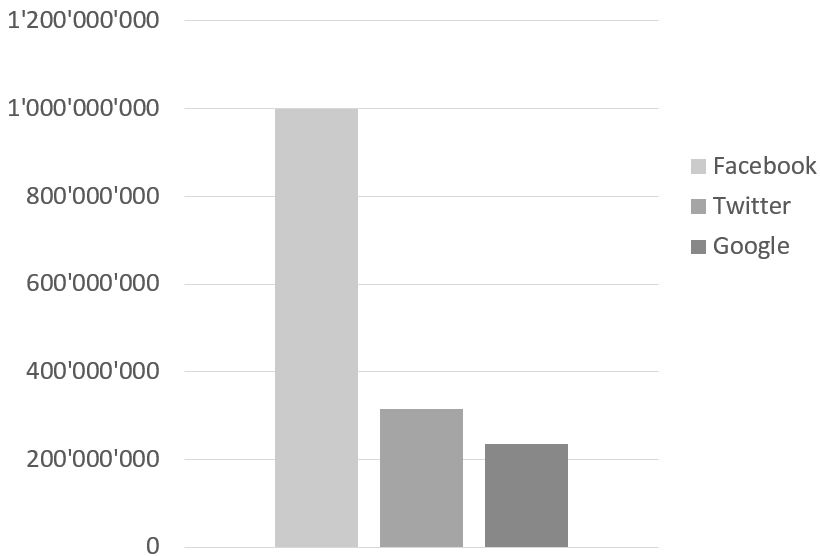
\includegraphics{images/excel-statistik/socialmedia-aktivenutzer.jpg}
\caption[Aktive Nutzer Weltweit]{Aktive Nutzer Weltweit\footnotemark{}}
\end{figure}
\footnotetext{Das Statistik wurde basierend auf den Daten von
  socialmedia-institute (``SMI (SocialMedia Institute)'' 2015)erstellt.
  Facebook und Twitter Daten sind am 5. November 2015 und die Google
  Daten sind im 2014 erhoben worden.}

Ganze \emph{78\%} (Interactive 2015) der Schweizer Bevölkerung nutzten
SocialMedia und besitzen dadurch einen OAuth-Account:

\begin{figure}[htbp]
\centering
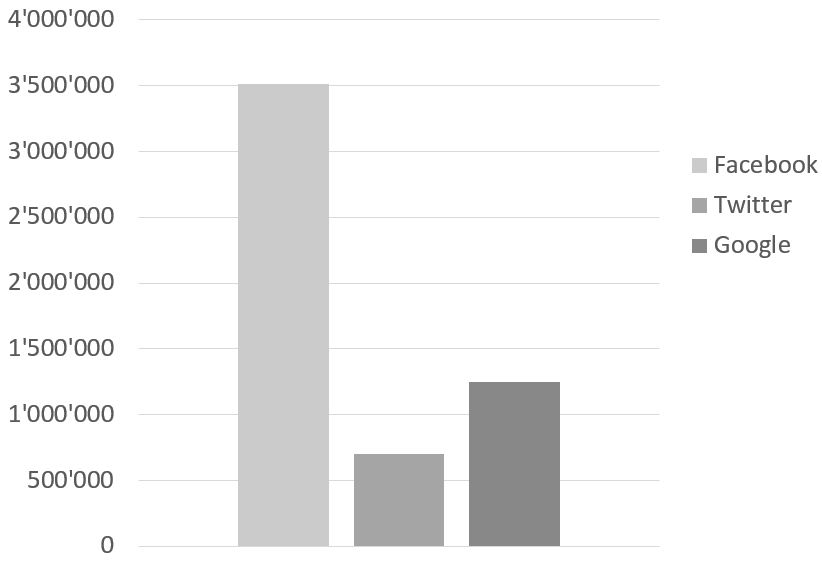
\includegraphics{images/excel-statistik/socialmedia-schweiz.jpg}
\caption[Anzahl Schweizer Nutzer]{Anzahl Schweizer
Nutzer\footnotemark{}}
\end{figure}
\footnotetext{Das Statistik wurde basierend auf den Daten von Goldbach
  Interactive (Interactive 2015) generiert. Die Daten sind im März 2015
  erhoben.}

\newpage

\subsubsection{Vorteile}\label{vorteile}

78\% der Schweizer Bevölkerung besitzt bereits einen OAuth Account. Das
Protokoll ist ein etablierter Standard.

\subsubsection{Nachteile}\label{nachteile}

Mehrfachregistrierungen sind möglich. Jenach OAuth-Provider werden
verschiedene Daten zur Verfügung gestellt. Pro OAuth Provider kann man
sich registrieren einen Abgleich der verschiedenen OAuth Provider wird
vom \protect\hyperlink{oauth}{OAuth}-Protokoll nicht zur Verfügung
gestellt. 22\% der Bevölkerung müsste sich vor Nutzung noch
registrieren. Die Implementierung ist trotz vielen Libaries nicht ohne
tiefere Programmierkenntnisse möglich.

\newpage

\subsection{playbuzz.com}\label{playbuzz.com}

Youtube von Google ist im Jahr 2015 mit Abstand die meist verbreiteste
(``Statistik Plattform'' 2015) Videopublishing-Plattform. Medienhäuser
nutzen Youtube um einfach Ihren Artikel mit einem Video zu ergänzen.
Neben der einfachen Integration profitieren die Medienhäuser von der
zusätzlichen Verbreitung über youtube.com und der einfachen viralen
Verbreitungsmöglichkeiten von youtube. PlayBuzz möchte das Youtube für
Votings, Quiz und ähnlicher Embeded Content zu werden. Neben MTV, Focus,
Time oder Bild verwendet seit Herbst 2015 auch ein grosses Medienhaus
der Schweiz die Plattform. Tamedia erfasst neu auf 20minuten Votings und
Umfragen mit PlayBuzz.

2012 wurde Playbuzz von Shaul Olmert (Sohn des Premie Minster von Israel
Ehuad Olmert) und Tom Pachys ins Leben gerufen. Der offizielle Launch
war im Dezember 2013. Im Juni 2014 wurde Playbuzz bereits das 1. Mal
unter den Top 10 Facebook Shared Publishers aufgelistet. Im Juni 2014
konnte Playbuzz bereits 70 millionen unique views aufweisen. Im
September 2014 kamen 7 von den 10 Top Shares auf Facebook laut
forbes.com von Playbuzz. Playbuzz setzt nach eigenen Angaben auf Content
wie Votes und Quizes welcher gerne Viral geteilt wird und ermöglicht
Endnutzer und Redaketeueren einfache Verwendung. (``Interview Mit Shaul
Olmert'' 2015) (``PlayBuzz'' 2015)

\subsubsection{Vorteile}\label{vorteile-1}

Playbuzz ist kostenlos und lässt sich einfach integrieren. Durch
Verwendung von Playbuzz kann die Verbreitung des eigenen Inhalts stark
gesteigert werden. Die Verwaltungsoberfläche und Reports sind
übersichtlich und einfach zu bedienen.

\subsubsection{Nachteile}\label{nachteile-1}

Der Verweis auf Playbuzz ist ersichtlich. Auch beim Posten auf den
SocialMedia-Kanälen ist die Herkunft von Playbuzz offensichtlich. Die
Möglichkeiten in Funktionalität und Design haben Grenzen. Individuelle
Erweiterungen sind nicht einfach möglich.

\newpage

\section{Grundlegende
Sicherheitskonzepte}\label{grundlegende-sicherheitskonzepte}

In diesem Unterkapitel werden die Grundlagen der Sicherheitskonzepte
vermittelt auf denen danach eine Authentifizierungssoftware aufgebaut
werden kann.

\subsection{KISS}\label{kiss}

\textbf{K}eep \textbf{I}t \textbf{S}tupid \emph{and} \textbf{S}imple

Ein verbreitetes Problem unter Software Engineers und Programmier heute
ist, dass sie dazu tendieren Probleme zu kompliziert und verschachtelt
zu lösen. 8-9 von 10 Entwickeln machen den Fehler, Probleme zu wenig
auseinander zu brechen und alles in einem grossen Programm zu lösen.
Anstatt es in kleinen Paketen verständlich zu
programmieren.(\textbf{???})

Software Entwickler profitieren von Kiss: - You will be able to solve
more problems, faster. - You will be able to produce code to solve
complex problems in fewer lines of code - You will be able to produce
higher quality code - You will be able to build larger systems, easier
to maintain - You're code base will be more flexible, easier to extend,
modify or refactor when new requirements arrive - You will be able to
achieve more than you ever imagined - You will be able to work in large
development groups and large projects since all the code is stupid
simple

\newpage

\ldots{}is really just ordinary text, \emph{plain and simple}. How is it
good for you?

\begin{itemize}
\tightlist
\item
  You just \textbf{type naturally}, and the result looks good.
\item
  You \textbf{don't have to worry} about clicking formatting buttons.
\item
  Or fiddling with indentation. (Two spaces is all you need.)
\end{itemize}

To see what else you can do with Markdown (including \textbf{tables},
\textbf{images}, \textbf{numbered lists}, and more) take a look at the
\href{https://github.com/adam-p/markdown-here/wiki/Markdown-Here-Cheatsheet}{Cheatsheet}.
And then try it out by typing in this box!

\begin{longtable}[c]{@{}rlcl@{}}
\toprule
Right & Left & Center & Default\tabularnewline
\midrule
\endhead
12 & 12 & 12 & 12\tabularnewline
123 & 123 & 123 & 123\tabularnewline
1 & 1 & 1 & 1\tabularnewline
\bottomrule
\end{longtable}

\begin{figure}[htbp]
\centering
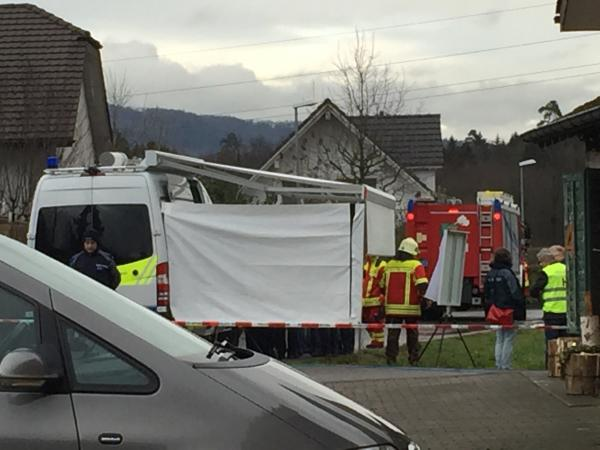
\includegraphics{images/image.jpg}
\caption{This is the caption}
\end{figure}

\begin{longtable}[c]{@{}lll@{}}
\toprule
Test & test2 & saleti\tabularnewline
\midrule
\endhead
olé & Thats the way\tabularnewline
\tabularnewline
\bottomrule
\end{longtable}

This is the day

\newpage

\chapter{Grundlagen}\label{grundlagen}

Dieses Kapitel erläutert die Grundlagen. Ein grosser Teil der Arbeit
stützt sich auf den Grundlagen ab (Meier 2010, 7:105)

\section{Basisbegriffe}\label{basisbegriffe}

\hypertarget{authentifizierung-1}{\subsection{Authentifizierung}\label{authentifizierung-1}}

\subsection{Autorisierung}\label{autorisierung-1}

Saleti

\newpage

\hypertarget{glossar}{\chapter{Glossar}\label{glossar}}

\textbf{ORM} ORM steht für object-relational mapping und ist eine
Technik mit der Objekte einer Anwendung in einem relationalen
Datenbanksystem abgelegt werden kann.\\
\textbf{Node} Node oder Node.js ist eine Plattform welche es erlaubt
JavaScript serverseitig auszuführen. \url{https://nodejs.org/}\\
\textbf{RPC} Remote Procedure Call ist eine Technologie um
Funktionsbausteine in einem anderen Prozess aufzurufen.\\
\textbf{Jasmine} Jasmine ist ein verhaltensbasiertes Testframework für
JavaScript. \url{http://jasmine.github.io}\\
\textbf{Karma} Karma ist ein Testrunner-Framework zur kontinuierlichen
Ausführung von UnitTests. \url{http://karma-runner.github.io}\\
\textbf{Mocks} Mocks sind Code-Attrappen, die es ermöglichen, noch nicht
vorhandene oder nicht verfügbare, Funktionalitäten und Objekte zu
simulieren. \url{http://de.wikipedia.org/wiki/Mock-Objekt}\\
\textbf{Github} Github ist ein Cloud basierter SourceCode
Verwaltungsdienst für Git. \url{https://github.com}

\chapter{Verzeichnisse}\label{verzeichnisse}

Neues Verzeichnisse

\section{Abbildungsverzeichnis}\label{abbildungsverzeichnis}

\renewcommand{\listfigurename}{} 

\begingroup\let\clearpage\relax
\listoffigures
\endgroup

\pagebreak

\section{Quellenverzeichnis}\label{quellenverzeichnis}

\renewcommand{\bibname}{}

\begingroup \let\clearpage\relax

\endgroup

\pagebreak

\section{Tabellenverzeichnis}\label{tabellenverzeichnis}

\renewcommand{\listtablename}{} 

\begingroup \let\clearpage\relax
\listoftables
\endgroup

\hypertarget{refs}{}
\hypertarget{ref-captcha}{}
Burling, Stacey. 2012. ``CAPTCHA: The Story Behind Those Squiggly
Computer Letters.''
\url{http://phys.org/news/2012-06-captcha-story-squiggly-letters.html}.

\hypertarget{ref-duden}{}
\emph{Duden}. 2014. Vol. 26. Dudenredaktion.

\hypertarget{ref-authentifizierungsdeforg}{}
``Http://authentifizierung.org.'' 2015.
\url{http://authentifizierung.org/}.

\hypertarget{ref-goldbachsocial}{}
Interactive, Goldbach. 2015. ``Nutzerzahlen Der Wichtigsten
Plattformen.'' \url{https://twitter.com/revogt/}.

\hypertarget{ref-t3nplaybuzz}{}
``Interview Mit Shaul Olmert.'' 2015.
\url{https://www.youtube.com/watch?v=X_fQ1uG9rFY}.

\hypertarget{ref-comescore-mobiletrends}{}
Lipsman, Andrew. 2014. ``Major Mobile Milestones in May: Apps Now Drive
Half of All Time Spent on Digital.''
\url{http://www.comscore.com/Insights/Blog/Major-Mobile-Milestones-in-May-Apps-Now-Drive-Half-of-All-Time-Spent-on-Digital}.

\hypertarget{ref-rupDatenbanken}{}
Meier, Andreas. 2010. \emph{Relationale Und Postrelationale
Datenbanken}. Vol. 7. EXamen.pressSpringerLink. Berlin, Heidelberg:
Springer Berlin Heidelberg.

\hypertarget{ref-playbuzz}{}
``PlayBuzz.'' 2015. \url{http://www.playbuzz.com}.

\hypertarget{ref-googlecaptcha}{}
``ReCAPTCHA Digitization Accuracy.'' 2014.
\url{http://www.google.com/recaptcha/digitizing}.

\hypertarget{ref-authentifizierungsdef}{}
Rouse, Margaret. 2015. ``Authentifizierung - Definition.''
\url{http://www.searchsecurity.de/definition/Authentifizierung}.

\hypertarget{ref-smi}{}
``SMI (SocialMedia Institute).'' 2015.
\url{http://socialmedia-institute.com/}.

\hypertarget{ref-statista}{}
``Statistik Plattform.'' 2015. \url{http://de.statista.com/}.


\end{document}